% !TEX TS-program = pdflatex
% !TEX encoding = UTF-8 Unicode

%************************************************
\chapter{Algoritmica e diffusione}
\label{chp:Algoritmica e Diffusione}
%************************************************

\epigraph{<<Comporre vuol dire \textit{costruire} uno strumento>> \\ \textbf{Helmut Lachenmann}}

In quest'ultimo capitolo visioneremo le modalità di riproduzione dei due movimenti, ma soprattutto un fattore esplicato in precedenza molto importante per quanto riguarda la riproducibilità di una composizione: \textit{la trasportabilità}. Ogni composizione deve essere, a mio parere, soprattutto nel caso di commissioni, trasportabile da una piattaforma all'altra, da una DAW all'altra, ma soprattutto avere dei parametri da essere riproducibile anche senza il compositore presente. \\
Per quanto riguarda L'albe nei varchi, il metodo ideato è proprio questo: il brano è riproducibile anche mono e gli effetti che vengono aggiunto nell'elaborazione, ovvero i riverberi, possono essere utilizzati anche direttamente in un live elettronics \textit{in loco}.


\section{Legenda e algoritmica}

I due varchi hanno due algoritmi differenti. Nel primo abbiamo degli inviluppi segnati in partitura e tre riverberi differenti, così da avere tre dimensioni differenti per ogni parte: il tape, l'elaborazione del sassofono soprano e la modulazione ad anello.

\begin{figure}

\begin{center}

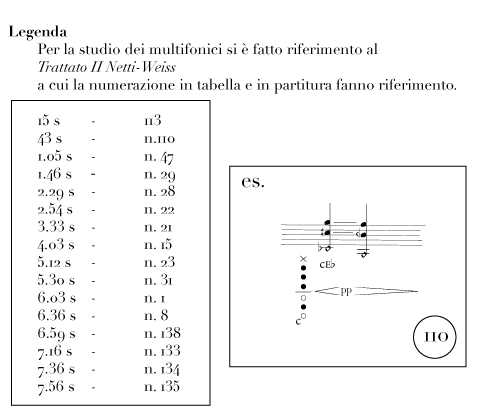
\includegraphics[width=1.\textwidth]{legenda_particolare_01.png}

\caption{particolare partitura \textit{Legenda, I Varco: L'albe}}

\label{fig:02_Algoritmo_01}

\end{center}

\end{figure}


\begin{figure}

\begin{center}

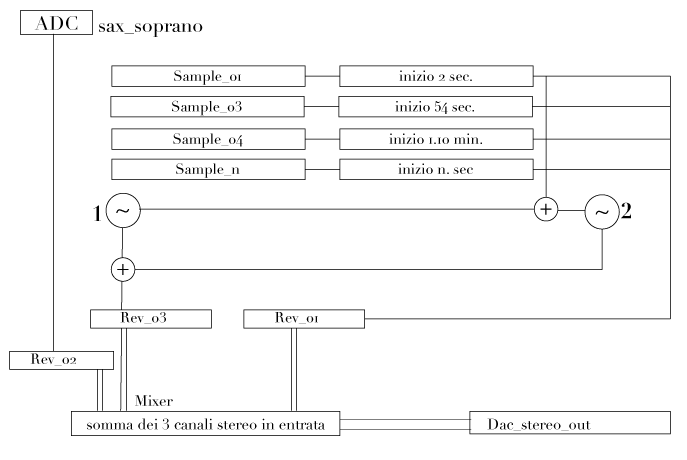
\includegraphics[width=1.\textwidth]{algoritmo_particolare_01.png}

\caption{particolare partitura \textit{Algoritmo I Varco: L'albe}}

\label{fig:02_Algoritmo_01}

\end{center}

\end{figure}


%************************************************

\section{Sistema di ripresa}

Il sistema di ripresa, date le condizioni di quarantena imposte dal decreto ministeriale dovuto al COVID-19, ho contattato il mio strumentista, Danilo Perticaro, e abbiamo optato per registrare in una piccola stanza con un microfono Zoom con ripresa stereo. I files mi sono stati inviati tutti a 44.1 kHz a 24bit. \\
Nel secondo varco, la ripresa microfonica, come esplicato nel capitolo 2, ho unito tre fonti sonore differenti presenti su Unamolla: 2 doppi humbucker e un piezoelettrico. Il tutto elaborato.

%************************************************

\section{Diffusione ambisonic} 

Le due composizioni, per quanto riguarda la riproduzione, erano state pensate per essere diffusione con più speaker. Purtroppo, data la situazione di emergenza non c'è stata la possibilità di farsi che questo avvenga e la soluzione è stata optare per due cambiamenti. Il brano \textit{L'albe} è diventato per diffusione stereo. In precedenza la mia idea era di utilizzare tre microfoni differenti e collocarli digitalmente, ognuno in una posizione diversa, modificando l'elevazione delle fonti, per dare una forma conica verso l'alto del suono del sassofono tenore. Tutta l'elettronica sarebbe stata collocata in tutti e 23 i diffusori della cupola e missata assieme al riverbero dedicato al sassofono che, come si può vedere in partitura, viene usato a livello compositivo, come gesto di continuazione dei multifonici del sassofono. \\
\textit{Insinuarsi nel vuoto, mosso contrario} invece, tramite decodifica \textit{binaurale} è stato trasformato per un ascolto in cuffia.  

\subsection{cupola di diffusori}
 
Entrambe le composizioni erano state ideate per essere riprodotte all'interno della cupola sonora presente nell'aula I, l'Aula Bianchini, al terzo piano del Conservatorio Santa Cecilia in Roma. Per via del cambiamento delle modalità di laurea, i brani sono rimasti entrambi in stereo. La decodifica ambisonic è stata sostituita da un ascolto frontale, stereofonico come si presenta negli algoritmi di costruzione. \\